% XeLaTeX, UTF-8. Bien dich hai lan de cap nhat muc luc va tham chieu.
% xelatex -interaction=nonstopmode -halt-on-error bao_cao_encoder_decoder_le_viet_thanh.tex
\documentclass[11pt,a4paper]{article}
\usepackage[top=2.35cm,bottom=2.3cm,left=2.4cm,right=2.4cm]{geometry}
\usepackage{fontspec}
\IfFontExistsTF{Times New Roman}{\setmainfont{Times New Roman}}{\setmainfont{TeX Gyre Termes}}
\IfFontExistsTF{Arial}{\setsansfont{Arial}}{\setsansfont{TeX Gyre Heros}}
\IfFontExistsTF{Consolas}{\setmonofont{Consolas}[Scale=0.84]}{\setmonofont{Latin Modern Mono}[Scale=0.84]}
\usepackage{amsmath,amssymb,bm}
\usepackage{booktabs,tabularx,longtable,array}
\usepackage[table]{xcolor}
\usepackage{graphicx,tikz}
\usetikzlibrary{arrows.meta,positioning,calc,fit,backgrounds}
\usepackage{titlesec,enumitem,setspace,fancyhdr,lastpage}
\usepackage{caption,float,listings,needspace}
\usepackage{hyperref}
\definecolor{ReportBlue}{HTML}{125BA0}
\definecolor{DeepBlue}{HTML}{173B61}
\definecolor{PaleBlue}{HTML}{EEF5FC}
\definecolor{Accent}{HTML}{27A2C4}
\definecolor{Ink}{HTML}{22313F}
\definecolor{Muted}{HTML}{53677A}
\hypersetup{colorlinks=true,linkcolor=ReportBlue,citecolor=ReportBlue,urlcolor=ReportBlue,
  pdftitle={Kiến trúc Encoder--Decoder trong xử lý ngôn ngữ tự nhiên},
  pdfauthor={Lê Việt Thành},pdfsubject={Seq2Seq, RNN, LSTM, GRU, Attention và Transformer},
  bookmarksnumbered=true}
\urlstyle{same}
\titleformat{\section}{\Large\bfseries\color{ReportBlue}}{\thesection.}{0.55em}{}
\titleformat{\subsection}{\large\bfseries\color{ReportBlue}}{\thesubsection.}{0.55em}{}
\titleformat{\subsubsection}{\normalsize\bfseries\color{ReportBlue}}{\thesubsubsection.}{0.55em}{}
\titlespacing*{\section}{0pt}{19pt}{9pt}
\titlespacing*{\subsection}{0pt}{13pt}{6pt}
\titlespacing*{\subsubsection}{0pt}{10pt}{4pt}
\setcounter{secnumdepth}{3}
\setcounter{tocdepth}{2}
\setstretch{1.16}
\setlength{\parindent}{0pt}
\setlength{\parskip}{5pt}
\setlength{\headheight}{15pt}
\setlength{\emergencystretch}{2em}
\setlength{\tabcolsep}{5pt}
\renewcommand{\arraystretch}{1.2}
\renewcommand{\contentsname}{Mục lục}
\renewcommand{\figurename}{Hình}
\renewcommand{\tablename}{Bảng}
\renewcommand{\refname}{Tài liệu tham khảo}
\captionsetup{font=small,labelfont={bf,color=ReportBlue},skip=7pt}
\setlist[itemize]{leftmargin=1.4em,itemsep=3pt,topsep=4pt}
\setlist[enumerate]{leftmargin=1.7em,itemsep=3pt,topsep=4pt}
\pagestyle{fancy}
\fancyhf{}
\fancyhead[L]{\small\color{Muted}ENCODER--DECODER / SEQ2SEQ}
\fancyhead[R]{\small\color{Muted}Lê Việt Thành}
\fancyfoot[L]{\small\color{Muted}Báo cáo chuyên đề}
\fancyfoot[R]{\small\color{ReportBlue}\thepage}
\renewcommand{\headrulewidth}{0.4pt}
\renewcommand{\footrulewidth}{0pt}
\numberwithin{equation}{section}
\newcolumntype{Y}{>{\raggedright\arraybackslash}X}
\newcommand{\R}{\mathbb{R}}
\newcommand{\BOS}{\langle\mathrm{BOS}\rangle}
\newcommand{\EOS}{\langle\mathrm{EOS}\rangle}
\newcommand{\PAD}{\langle\mathrm{PAD}\rangle}
\newcommand{\UNK}{\langle\mathrm{UNK}\rangle}
\newcommand{\softmax}{\operatorname{softmax}}
\newcommand{\concat}{\operatorname{concat}}
\newcommand{\notebox}[2]{\par\smallskip\noindent
  \begingroup\setlength{\fboxsep}{10pt}\colorbox{PaleBlue}{%
  \parbox{\dimexpr\linewidth-20pt\relax}{\textbf{\color{ReportBlue}#1}\par\smallskip #2}}%
  \endgroup\par\smallskip}
\lstset{language=Python,basicstyle=\ttfamily\small\linespread{1}\selectfont,keywordstyle=\color{ReportBlue}\bfseries,
  commentstyle=\color{Muted},stringstyle=\color{DeepBlue},backgroundcolor=\color{PaleBlue},
  frame=single,rulecolor=\color{ReportBlue!20},breaklines=true,columns=fullflexible,
  keepspaces=true,showstringspaces=false,numbers=left,numberstyle=\tiny\color{Muted},
  numbersep=7pt,xleftmargin=14pt,framexleftmargin=9pt,aboveskip=9pt,belowskip=9pt,
  tabsize=4}
\tikzset{block/.style={draw=ReportBlue,fill=PaleBlue,rounded corners=3pt,
  minimum height=1.05cm,align=center,font=\small,inner sep=6pt},
  arr/.style={-{Latex[length=2.5mm]},thick,draw=ReportBlue},
  tinyblock/.style={draw=ReportBlue,fill=PaleBlue,rounded corners=2pt,
  minimum width=1.4cm,minimum height=0.65cm,align=center,font=\small}}

\begin{document}
\color{Ink}
\begin{titlepage}
\begin{tikzpicture}[remember picture,overlay]
  \fill[DeepBlue] (current page.north west) rectangle ([xshift=1.2cm]current page.south west);
  \fill[PaleBlue] ([xshift=1.2cm,yshift=-1.8cm]current page.north west)
    rectangle ([yshift=-6.6cm]current page.north east);
  \draw[Accent,line width=3pt] ([xshift=2.4cm,yshift=-2.2cm]current page.north west)
    -- ([xshift=5.4cm,yshift=-2.2cm]current page.north west);
\end{tikzpicture}
\vspace*{1.0cm}
{\sffamily\small\bfseries\color{ReportBlue}BÁO CÁO CHUYÊN ĐỀ\par}
\vspace{0.65cm}
{\sffamily\fontsize{28}{34}\selectfont\bfseries\color{DeepBlue}
KIẾN TRÚC\par ENCODER--DECODER\par}
\vspace{0.3cm}
{\sffamily\Large\color{ReportBlue}Trong xử lý ngôn ngữ tự nhiên\par}
\vspace{1.5cm}
{\Large\bfseries Từ Sequence-to-Sequence đến\par Attention và Transformer\par}
\vspace{0.55cm}
{\large Cơ sở toán học, cơ chế hoạt động,\par huấn luyện, suy luận và đánh giá\par}
\vspace{1.4cm}
{\color{ReportBlue}\rule{\linewidth}{0.8pt}}\par
\vspace{0.4cm}
{\large Trình bày: \textbf{Lê Việt Thành}\par}
\vspace{0.35cm}
{\normalsize Ngày hoàn thành: 09 tháng 10 năm 2026\par}
\vfill
\begin{tikzpicture}[node distance=0.45cm]
\node[block,text width=3.1cm] (a) {Chuỗi đầu vào\\$x_1,\ldots,x_T$};
\node[block,text width=3.3cm,right=of a] (b) {Biểu diễn ngữ cảnh\\$c$ hoặc $H$};
\node[block,text width=3.1cm,right=of b] (c) {Chuỗi đầu ra\\$y_1,\ldots,y_U$};
\draw[arr] (a) -- (b); \draw[arr] (b) -- (c);
\end{tikzpicture}\par
\vspace{0.6cm}
{\small\color{Muted}Tổng hợp từ các nguồn được chỉ định, giáo trình Dive into Deep Learning\par
và các công trình nghiên cứu gốc. Các ví dụ số và sơ đồ được xây dựng để minh họa.\par}
\end{titlepage}

\pagenumbering{roman}
\section*{Tóm tắt}
\addcontentsline{toc}{section}{Tóm tắt}
Kiến trúc Encoder--Decoder tổ chức mô hình thành hai khối: encoder tạo biểu diễn từ đầu vào và decoder sử dụng biểu diễn đó để tạo đầu ra. Trong bài toán Sequence-to-Sequence (Seq2Seq), đầu vào và đầu ra là các chuỗi có độ dài có thể khác nhau. Báo cáo tập trung vào xử lý ngôn ngữ tự nhiên, đặc biệt là dịch máy, để giải thích mối liên hệ giữa biểu diễn ngôn ngữ và sinh chuỗi có điều kiện.

Nội dung đi từ mô hình hồi quy dùng một vector ngữ cảnh đến cơ chế Attention và kiến trúc Transformer. Các phần chính làm rõ token hóa, embedding, trạng thái ẩn, xác suất chuỗi, hàm mất mát cross-entropy, teacher forcing, các loại mask và thuật toán giải mã. Ví dụ Anh--Việt được dùng xuyên suốt để đối chiếu giữa công thức và luồng dữ liệu. Báo cáo cũng cung cấp một thiết kế thực nghiệm, bảng phân tích lỗi và mã PyTorch minh họa mô hình GRU.

Đây là \textbf{báo cáo tổng quan lý thuyết và hướng dẫn triển khai}. Các xác suất, trọng số Attention và cấu hình thí nghiệm minh họa không phải kết quả huấn luyện thực tế. Các kết quả lịch sử nếu được nhắc đến đều gắn với công trình gốc và bối cảnh đánh giá của công trình đó.

\textbf{Từ khóa:} Encoder--Decoder; Seq2Seq; RNN; LSTM; GRU; Attention; Transformer; dịch máy; teacher forcing.

\subsection*{Mục tiêu và cách đọc}
Sau khi đọc báo cáo, người học cần có khả năng:
\begin{enumerate}
\item Mô tả chính xác dữ liệu nào đi vào encoder, dữ liệu nào đi vào decoder và đầu ra của từng khối.
\item Giải thích vì sao decoder phải nhận token của bước trước, và vì sao huấn luyện khác với suy luận.
\item Viết được các phương trình cơ bản của Seq2Seq và xác định kích thước tensor.
\item Phân biệt vector ngữ cảnh cố định, Attention theo bước và cross-attention trong Transformer.
\item Thiết kế quy trình đánh giá có thể tái lập và nhận diện các lỗi triển khai thường gặp.
\end{enumerate}
Người mới nên đọc các mục 1--5 trước; các mục 6--9 mở rộng cơ chế; các mục 10--12 và phụ lục hỗ trợ triển khai, thực nghiệm và ôn tập.
\clearpage
\begingroup
\setstretch{1.10}
\setlength{\parskip}{0pt}
\normalsize
\tableofcontents
\endgroup
\clearpage
\pagenumbering{arabic}

\section{Giới thiệu và phạm vi kiến trúc}
\subsection{Vấn đề ánh xạ giữa hai chuỗi}
Trong dịch máy, một câu nguồn không chỉ được thay từng từ bằng từ đích. Mô hình còn phải xử lý khác biệt về trật tự, hình thái và cách diễn đạt. Chẳng hạn, ``I love machine learning'' có thể được dịch thành ``Tôi yêu thích học máy''. Nếu token hóa theo khoảng trắng thì câu nguồn có bốn token và câu đích có năm token nội dung. Với một tokenizer subword, cả hai độ dài có thể thay đổi tiếp.

Một mô hình phù hợp cần nhận chuỗi dài ngắn khác nhau, khai thác toàn bộ ngữ cảnh nguồn và tạo đầu ra cho đến khi hoàn thành ý nghĩa. Encoder--Decoder cung cấp cách phân chia công việc này: đọc và biểu diễn đầu vào, sau đó sinh đầu ra có điều kiện. Trong giáo trình D2L, decoder được diễn giải như một mô hình ngôn ngữ có điều kiện trên biểu diễn nguồn và tiền tố đích~\cite{d2larch}.

\subsection{Encoder và decoder trong bài toán Seq2Seq}
Trong báo cáo này, \textbf{Encoder--Decoder} được xét trực tiếp cho bài toán \textbf{Seq2Seq trong NLP}: một chuỗi văn bản nguồn được chuyển thành chuỗi văn bản đích. Encoder đọc các token nguồn và tạo biểu diễn ngữ cảnh; decoder dựa vào biểu diễn đó cùng các token đích trước để sinh token tiếp theo. Ví dụ xuyên suốt là dịch ``I love machine learning'' thành ``Tôi yêu thích học máy''.

\begin{table}[H]
\centering\small
\begin{tabularx}{\linewidth}{@{}p{3cm}YY@{}}
\toprule
\rowcolor{PaleBlue}Thành phần & Vai trò trong NLP & Ví dụ dịch Anh--Việt\\\midrule
Encoder & Đọc embedding nguồn bằng GRU/LSTM, tạo hidden state và các trạng thái theo vị trí. & Đọc I, love, machine, learning và EOS.\\
Decoder & Nhận BOS hoặc token đích trước đó, dùng ngữ cảnh nguồn để dự đoán token mới. & Từ BOS sinh Tôi, rồi yêu, thích, học, máy và EOS.\\
Seq2Seq & Học toàn bộ ánh xạ nguồn--đích bằng hai khối encoder và decoder. & Câu tiếng Anh bốn token sang câu tiếng Việt năm token nội dung.\\
\bottomrule
\end{tabularx}
\caption{Encoder và decoder phối hợp trong mô hình Seq2Seq dịch văn bản.}
\end{table}
\notebox{Cách hiểu chính xác}{``Mã hóa'' trong báo cáo là biến dữ liệu thành biểu diễn học được. Khái niệm này không chỉ hoạt động mã hóa bảo mật; decoder cũng không được bảo đảm khôi phục nguyên văn đầu vào.}

\subsection{Nguồn tài liệu và nguyên tắc tổng hợp}
Bài viết trên Trí tuệ nhân tạo cung cấp cách tiếp cận trực quan theo ba thành phần: encoder, vector trung gian và decoder~\cite{tritue}. Bài Number Analytics mở rộng góc nhìn sang nhiều kiểu đầu vào và ứng dụng~\cite{numberanalytics}. D2L cung cấp khung lý thuyết và cách tổ chức mô hình~\cite{d2larch}. Các công thức và mốc phát triển được đối chiếu với Sutskever và cộng sự, Cho và cộng sự, Bahdanau và cộng sự, cùng Vaswani và cộng sự~\cite{sutskever,cho,bahdanau,vaswani}.

Khi chuyển từ giới thiệu phổ thông sang mô hình NLP, cần điều chỉnh ba điểm: biểu diễn encoder không nhất thiết có chiều thấp hơn dữ liệu ban đầu; không phải mô hình nào cũng chỉ trả về một vector; và sinh token phân loại thường dùng cross-entropy thay vì sai số bình phương trên token ID. Báo cáo dùng các phân biệt này xuyên suốt để tránh suy rộng mô hình cơ bản sang mọi biến thể.

\section{Biểu diễn dữ liệu và cơ sở xác suất}
\subsection{Ký hiệu thống nhất}
\begin{table}[H]
\centering\small
\begin{tabularx}{\linewidth}{@{}p{3cm}Y@{}}
\toprule\rowcolor{PaleBlue}Ký hiệu & Ý nghĩa\\\midrule
$x=(x_1,\ldots,x_T)$ & Chuỗi token nguồn có độ dài hợp lệ $T$.\\
$y=(y_1,\ldots,y_U)$ & Chuỗi token đích gồm $U$ token nội dung; đặt $y_{U+1}=\EOS$.\\
$y_{<t}$ & Các token đích trước vị trí $t$; decoder bắt đầu bằng $y_0=\BOS$.\\
$V_s,V_t$ & Kích thước từ vựng nguồn và đích.\\
$d_e,d_h,d_s$ & Chiều embedding, trạng thái encoder và trạng thái decoder.\\
$h_i,s_t$ & Trạng thái ẩn encoder tại $i$ và decoder tại $t$.\\
$c,H,c_t$ & Ngữ cảnh cố định, tập trạng thái nguồn và ngữ cảnh Attention tại bước $t$.\\
$\theta$ & Toàn bộ tham số học được của mô hình.\\
$B,m_{b,t}$ & Kích thước batch và mask đánh dấu nhãn hợp lệ.\\
\bottomrule
\end{tabularx}
\caption{Ký hiệu sử dụng trong báo cáo.}
\end{table}
Các phương trình RNN trong báo cáo dùng \textbf{vector cột}. Trong mã PyTorch, các tensor được lưu theo trục batch và trục chuỗi, nên thứ tự các phép nhân trong cài đặt có thể trông khác nhưng vẫn biểu diễn cùng ánh xạ.

\subsection{Từ văn bản đến token và embedding}
Quy trình tiền xử lý gồm chuẩn hóa Unicode, tách token, ánh xạ token sang ID và tạo batch. Token có thể là từ, âm tiết, ký tự hoặc subword. Với tiếng Việt, khoảng trắng thường phân tách âm tiết; một từ như ``trí tuệ'' có thể gồm nhiều đơn vị nếu tách theo khoảng trắng. Vì vậy, độ dài chuỗi phải được hiểu theo tokenizer đã chọn, không phải luôn theo số từ ngôn ngữ học.

Cho ma trận embedding nguồn $E_s\in\R^{V_s\times d_e}$, embedding của token $x_i$ là
\begin{equation}
e_i=E_s[x_i,:]^{\mathsf T}\in\R^{d_e}.
\end{equation}
ID chỉ là vị trí tra cứu trong bảng. Ví dụ ID 100 không mang ý nghĩa ngôn ngữ lớn gấp đôi ID 50. Quan hệ ngữ nghĩa hình thành từ các vector học được và cách mô hình sử dụng chúng. Encoder và decoder có thể có embedding riêng; việc chia sẻ embedding đòi hỏi từ vựng và kích thước tương thích.

Subword giúp biểu diễn nhiều từ hiếm bằng các mảnh đã biết. Công trình của Sennrich và cộng sự đưa cách dùng đơn vị subword vào dịch máy nơ-ron, giảm phụ thuộc vào từ vựng nguyên khối~\cite{subword}. Tuy nhiên, tách nhỏ hơn thường làm chuỗi dài hơn; lựa chọn tokenizer còn ảnh hưởng chi phí tính toán và cách đo độ dài.

\begin{table}[H]
\centering\small
\begin{tabularx}{\linewidth}{@{}p{2.4cm}YY@{}}
\toprule\rowcolor{PaleBlue}Token & Vai trò & Quy tắc sử dụng\\\midrule
$\BOS$ & Khởi động decoder. & Đưa vào đầu chuỗi decoder; thường không nằm trong nhãn cần sinh.\\
$\EOS$ & Đánh dấu kết thúc. & Là nhãn hợp lệ, tham gia loss; dùng để dừng suy luận.\\
$\PAD$ & Bổ sung độ dài cho batch. & Bỏ qua trong loss; loại khỏi phần nguồn được Attention truy cập.\\
$\UNK$ & Biểu diễn token ngoài từ vựng nếu tokenizer cần. & Có thể làm mất tên riêng và chi tiết; không phải mọi tokenizer đều dùng.\\
\bottomrule
\end{tabularx}
\caption{Các token đặc biệt trong một thiết kế Seq2Seq cơ bản.}
\end{table}

\subsection{Phân phối có điều kiện của toàn chuỗi}
Với chuỗi đích đã thêm EOS, quy tắc dây chuyền cho phép viết
\begin{equation}\label{eq:factor}
p_\theta(y_1,\ldots,y_{U+1}\mid x)
=\prod_{t=1}^{U+1}p_\theta(y_t\mid y_{<t},x).
\end{equation}
Đây là xác suất của một chuỗi cụ thể. Mỗi thừa số là một phân phối trên từ vựng đích. EOS cho mô hình biểu diễn việc kết thúc ở những độ dài khác nhau. Việc phân rã xác suất không tự quy định phải dùng RNN hay Transformer; kiến trúc quyết định cách tính các phân phối thành phần.

Mục tiêu suy luận thường được viết
\begin{equation}
\hat y=\arg\max_y\log p_\theta(y\mid x)
=\arg\max_y\sum_t\log p_\theta(y_t\mid y_{<t},x).
\end{equation}
Không gian các chuỗi tăng rất nhanh theo từ vựng và độ dài. Vì vậy, greedy và beam search được dùng như cách tìm kiếm xấp xỉ. Ngoài xác suất mô hình, chất lượng cuối cùng còn phụ thuộc dữ liệu, mục tiêu huấn luyện và tiêu chí giải mã.

\section{Cấu trúc tổng thể của Encoder--Decoder}
\subsection{Ba thành phần và luồng thông tin}
\begin{figure}[H]
\centering
\begin{tikzpicture}[node distance=0.48cm]
\node[block,text width=2.4cm] (x) {Token nguồn\\$x_1,\ldots,x_T$};
\node[block,text width=2.5cm,right=of x] (enc) {Encoder\\Đọc và biểu diễn};
\node[block,text width=2.5cm,right=of enc] (ctx) {Ngữ cảnh\\$c$ hoặc $H$};
\node[block,text width=2.5cm,right=of ctx] (dec) {Decoder\\Sinh có điều kiện};
\node[block,text width=2.7cm,below=0.8cm of dec] (out) {Token đích và EOS\\$\hat y_1,\ldots,\hat y_U$};
\node[block,text width=3.1cm,below=0.8cm of ctx] (prefix) {Tiền tố đích\\$\BOS,y_1,\ldots,y_{t-1}$};
\draw[arr] (x) -- (enc); \draw[arr] (enc) -- (ctx); \draw[arr] (ctx) -- (dec);
\draw[arr] (dec) -- (out); \draw[arr] (prefix.east) -- (dec.south west);
\end{tikzpicture}
\caption{Luồng thông tin của Seq2Seq. Tiền tố đích dùng token đúng khi teacher forcing và token mô hình đã sinh khi suy luận. Sơ đồ do người viết xây dựng.}
\label{fig:overview}
\end{figure}
Encoder trả về biểu diễn phù hợp với decoder. Ở bản hồi quy cơ bản, biểu diễn có thể là trạng thái cuối $c=h_T$. Khi encoder là LSTM, trạng thái cuối còn gồm trạng thái ô nhớ. Khi có Attention, mô hình giữ nhiều trạng thái $H=(h_1,\ldots,h_T)$ thay vì chỉ một trạng thái tổng hợp. Với Transformer, $H$ thường là ma trận biểu diễn theo vị trí.

Decoder không chỉ biến một vector thành tất cả từ cùng lúc. Trong mô hình tự hồi quy, ở bước $t$ nó dựa vào biểu diễn nguồn và tiền tố đích để dự đoán phân phối cho token mới. Sau khi chọn token, tiền tố được kéo dài và quá trình lặp lại.

\subsection{Hai khối có cần cùng loại mạng không?}
Encoder và decoder đều xử lý token văn bản nhưng không bắt buộc có cấu hình giống nhau. Trong notebook \texttt{encode\_decode\_s2s.ipynb}, encoder dùng GRU hai chiều để đọc câu tiếng Anh; decoder dùng GRU một chiều để sinh câu tiếng Việt. Encoder trả các trạng thái theo vị trí cho Attention và một trạng thái khởi tạo decoder. Cặp GRU--GRU này thể hiện trực tiếp kiến trúc Seq2Seq trong NLP.

Nếu encoder hai chiều trả trạng thái có kích thước $2d_h$ còn decoder cần $d_s$, cần một phép chiếu, chẳng hạn
\begin{equation}
s_0=\tanh(W_{\mathrm{init}}[\overrightarrow h_T;\overleftarrow h_1]+b_{\mathrm{init}}),
\quad W_{\mathrm{init}}\in\R^{d_s\times 2d_h}.
\end{equation}
Phép chiếu này là tham số học được. Nó chuyển hình dạng và kết hợp thông tin; nó không bảo đảm giữ nguyên mọi chi tiết của câu nguồn.

\section{Seq2Seq dựa trên RNN, LSTM và GRU}
\subsection{Encoder RNN đọc chuỗi như thế nào?}
Với RNN đơn giản, đặt $h_0=0$ và tính
\begin{equation}\label{eq:rnn}
h_i=\tanh(W_xe_i+W_hh_{i-1}+b_h).
\end{equation}
Ở đây $W_x\in\R^{d_h\times d_e}$, $W_h\in\R^{d_h\times d_h}$ và $b_h\in\R^{d_h}$. Cùng bộ trọng số được dùng ở mọi vị trí. Trạng thái $h_i$ vừa phụ thuộc token hiện tại, vừa phụ thuộc thông tin đã tích lũy từ tiền tố nguồn.

\begin{figure}[H]
\centering
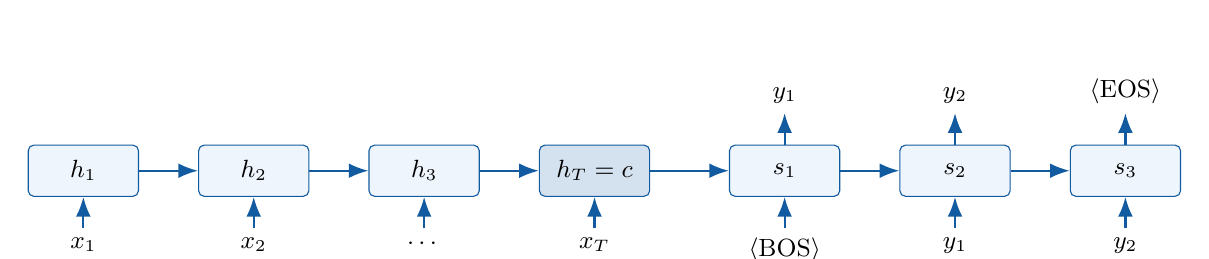
\begin{tikzpicture}[node distance=0.75cm]
\node[tinyblock] (h1) {$h_1$};
\node[tinyblock,right=of h1] (h2) {$h_2$};
\node[tinyblock,right=of h2] (h3) {$h_3$};
\node[tinyblock,right=of h3,fill=ReportBlue!18] (h4) {$h_T=c$};
\node[tinyblock,right=1.0cm of h4] (s1) {$s_1$};
\node[tinyblock,right=of s1] (s2) {$s_2$};
\node[tinyblock,right=of s2] (s3) {$s_3$};
\foreach \a/\b in {h1/h2,h2/h3,h3/h4,h4/s1,s1/s2,s2/s3}{\draw[arr] (\a)--(\b);}
\foreach \a/\v in {h1/x_1,h2/x_2,h3/\cdots,h4/x_T}{
  \node[below=0.4cm of \a,font=\small] (in\a) {$\v$};\draw[arr] (in\a)--(\a);}
\foreach \a/\v in {s1/y_1,s2/y_2,s3/\EOS}{
  \node[above=0.4cm of \a,font=\small] (out\a) {$\v$};\draw[arr] (\a)--(out\a);}
\node[below=0.4cm of s1,font=\small] (bos) {$\BOS$};\draw[arr] (bos)--(s1);
\node[below=0.4cm of s2,font=\small] (prev1) {$y_1$};\draw[arr] (prev1)--(s2);
\node[below=0.4cm of s3,font=\small] (prev2) {$y_2$};\draw[arr] (prev2)--(s3);
\end{tikzpicture}
\caption{RNN được trải theo thời gian. Mỗi khối là một lần áp dụng ô hồi quy với trọng số dùng chung; encoder và decoder có tham số riêng.}
\end{figure}
Trong batch có padding, ``trạng thái cuối'' phải được hiểu là trạng thái ở \textbf{cuối phần nguồn hợp lệ}. Nếu lấy trạng thái sau nhiều bước PAD, kết quả có thể bị biến đổi bởi hồi quy dù embedding PAD bằng không. Có thể xử lý bằng packed sequence hoặc chọn trạng thái tại độ dài thật theo cách nhất quán.

\subsection{Decoder và tầng phân phối token}
Một decoder cơ bản khởi tạo $s_0=g(c)$ và cập nhật
\begin{align}
s_t&=\tanh(U_ye^{(t)}_{t-1}+U_ss_{t-1}+b_s),\\
o_t&=W_os_t+b_o,\\
p_\theta(y_t=j\mid y_{<t},x)&=\frac{\exp(o_{t,j})}{\sum_{k=1}^{V_t}\exp(o_{t,k})}.
\end{align}
$e^{(t)}_{t-1}$ là embedding đích của token trước; $o_t\in\R^{V_t}$ là logits. Với chiều decoder $d_s$, $U_y\in\R^{d_s\times d_e}$ và $W_o\in\R^{V_t\times d_s}$. Một số thiết kế còn ghép $c$ vào đầu vào ở mỗi bước; đây là lựa chọn kiến trúc, không phải yêu cầu của mọi Seq2Seq.

Trong triển khai loss bằng PyTorch, đưa logits trực tiếp vào \texttt{CrossEntropyLoss}; hàm này đã bao gồm phép tính tương ứng với log-softmax~\cite{torchce}. Softmax tường minh chỉ cần khi muốn xem xác suất hoặc chọn token theo phân phối.

\subsection{Vì sao RNN đơn giản gặp khó với chuỗi dài?}
Gradient từ một bước muộn về bước sớm chứa tích của nhiều ma trận Jacobian. Nếu các hệ số liên tiếp làm co gradient, ảnh hưởng của thông tin xa giảm mạnh; nếu làm phóng đại gradient, cập nhật có thể mất ổn định. Từ phương trình~\eqref{eq:rnn}, có thể thấy các phép biến đổi được lặp nhiều lần theo thời gian. LSTM và GRU đưa cơ chế cổng vào đường truyền trạng thái để kiểm soát giữ và cập nhật thông tin.

\subsection{LSTM: trạng thái ẩn và trạng thái ô nhớ}
Gọi $q_i=[e_i;h_{i-1}]$, một dạng LSTM phổ biến là
\begin{align}
f_i&=\sigma(W_fq_i+b_f), & i_i&=\sigma(W_iq_i+b_i),\\
o_i&=\sigma(W_oq_i+b_o), & \tilde a_i&=\tanh(W_aq_i+b_a),\\
a_i&=f_i\odot a_{i-1}+i_i\odot\tilde a_i, & h_i&=o_i\odot\tanh(a_i).
\end{align}
$a_i$ là trạng thái ô nhớ, khác với ngữ cảnh $c$; $f_i,i_i,o_i$ là cổng quên, đầu vào và đầu ra; $\odot$ là tích theo phần tử. Khi khởi tạo decoder LSTM từ encoder LSTM, thường cần chuyển \textbf{cả} hidden state và cell state, hoặc học các phép chiếu thích hợp~\cite{d2llstm}. Thiết kế Seq2Seq của Sutskever và cộng sự dùng LSTM nhiều lớp cho cả hai khối~\cite{sutskever}.

\subsection{GRU: cơ chế cổng gọn hơn}
Với quy ước cổng cập nhật giữ trạng thái cũ khi gần 1, GRU có dạng
\begin{align}
r_i&=\sigma(W_re_i+U_rh_{i-1}+b_r),\\
z_i&=\sigma(W_ze_i+U_zh_{i-1}+b_z),\\
\tilde h_i&=\tanh(W_ne_i+U_n(r_i\odot h_{i-1})+b_n),\\
h_i&=z_i\odot h_{i-1}+(1-z_i)\odot\tilde h_i.
\end{align}
GRU không tách cell state riêng. Cổng reset tác động đến cách dùng trạng thái cũ khi tạo ứng viên; cổng update trộn ứng viên với trạng thái cũ~\cite{cho,d2lgru}. Có tài liệu dùng quy ước $z$ đảo chiều, nên cần đọc phương trình thay vì chỉ dựa vào tên cổng.

\notebox{Đối chiếu công thức với thư viện}{PyTorch áp dụng cổng reset sau phần biến đổi tuyến tính của hidden state trong phép tính ứng viên GRU. Vị trí này khác dạng $U_n(r_i\odot h_{i-1})$ ở trên. Hai dạng nói chung không tương đương; khi tái lập một mô hình cần ghi rõ biến thể~\cite{torchgru}.}

\subsection{So sánh các ô hồi quy}
\begin{table}[H]
\centering\small
\begin{tabularx}{\linewidth}{@{}p{2cm}YYY@{}}
\toprule\rowcolor{PaleBlue}Tiêu chí & RNN đơn giản & LSTM & GRU\\\midrule
Trạng thái & Một hidden state. & Hidden state và cell state. & Một hidden state.\\
Cơ chế cổng & Không có cổng tường minh. & Quên, đầu vào, đầu ra. & Reset và update.\\
Tham số một lớp & Xấp xỉ $h(d+h+1)$. & Xấp xỉ $4h(d+h+1)$. & Xấp xỉ $3h(d+h+1)$.\\
Ý nghĩa thực hành & Dễ quan sát cơ chế. & Kiểm soát bộ nhớ linh hoạt. & Cấu trúc gọn hơn LSTM cùng $d,h$.\\
\bottomrule
\end{tabularx}
\caption{Ước lượng với embedding đầu vào $d$, hidden size $h$ và một bias cho mỗi phép biến đổi cổng; thư viện có thể dùng hai bộ bias. Không suy ra chất lượng chỉ từ số tham số.}
\end{table}

\section{Ví dụ xuyên suốt: dịch câu Anh--Việt}
\subsection{Dữ liệu minh họa và cách dịch phải nhãn}
Xét câu nguồn ``I love machine learning'' và câu đích ``Tôi yêu thích học máy''. Trong phần này, chọn token hóa theo khoảng trắng để quan sát rõ từng bước. Khi đó
\begin{align*}
x&=(\text{I},\text{love},\text{machine},\text{learning}),\\
y^+&=(\text{Tôi},\text{yêu},\text{thích},\text{học},\text{máy},\EOS),\\
y^{\mathrm{in}}&=(\BOS,\text{Tôi},\text{yêu},\text{thích},\text{học},\text{máy}).
\end{align*}
Đầu vào decoder và nhãn có cùng số vị trí, nhưng lệch nhau một token. Decoder tại vị trí 1 nhìn BOS để dự đoán ``Tôi'', tại vị trí 2 nhìn ``Tôi'' để dự đoán ``yêu''.

\begin{table}[H]
\centering\small
\begin{tabularx}{\linewidth}{@{}cp{3.1cm}p{2.6cm}Y@{}}
\toprule\rowcolor{PaleBlue}Bước & Input khi huấn luyện & Nhãn & Input khi suy luận\\\midrule
1 & BOS & Tôi & BOS.\\
2 & Tôi thật & yêu & Token dự đoán bước 1.\\
3 & yêu thật & thích & Token dự đoán bước 2.\\
4 & thích thật & học & Token dự đoán bước 3.\\
5 & học thật & máy & Token dự đoán bước 4.\\
6 & máy thật & EOS & Token dự đoán bước 5.\\
\bottomrule
\end{tabularx}
\caption{Teacher forcing sử dụng token đúng ở bước trước, không sử dụng token cần dự đoán của bước hiện tại.}
\end{table}

\subsection{Một bước dự đoán bằng số}
Giả sử ở bước đầu decoder tạo xác suất trên ba token minh họa:
\begin{equation*}
p(\text{Tôi})=0.7,\quad p(\text{Bạn})=0.2,\quad p(\EOS)=0.1.
\end{equation*}
Nhãn đúng là ``Tôi'', nên loss bước này bằng $-\ln(0.7)\approx0.357$. Nếu ở bước sau xác suất của nhãn đúng ``yêu'' chỉ bằng $0.4$, loss tương ứng là $-\ln(0.4)\approx0.916$. Mô hình bị phạt mạnh hơn khi phân phối gán ít xác suất cho nhãn đúng.

Với logits $o$ và one-hot label $q$, đạo hàm cross-entropy theo logits là
\begin{equation}
\frac{\partial\ell}{\partial o_j}=p_j-q_j.
\end{equation}
Ở token ``Tôi'', giá trị là $0.7-1=-0.3$; ở ``Bạn'' là $0.2-0=0.2$. Kết hợp với gradient qua các tầng trước, cập nhật tham số theo hướng giảm loss sẽ điều chỉnh logits và các biểu diễn tạo ra chúng. Đây là \textbf{phép tính giả định} để giải thích gradient, không phải đầu ra của mô hình đã huấn luyện.

\subsection{Tại sao không có ánh xạ một--một giữa các vị trí?}
Cụm ``machine learning'' có thể tương ứng với ``học máy'', và một lựa chọn diễn đạt khác có thể là ``học tập máy''. Decoder cần quyết định cách diễn đạt toàn chuỗi thay vì gán cố định một token nguồn cho một token đích. Attention hỗ trợ truy cập thông tin liên quan ở từng bước nhưng không bắt buộc phải tạo phép căn chỉnh một--một.

Nếu câu đích có nhiều cách dịch đúng, dữ liệu huấn luyện thường chỉ cung cấp một hoặc một số câu tham chiếu. Loss token đo độ phù hợp với nhãn được cung cấp; nó không liệt kê đầy đủ mọi cách diễn đạt hợp lệ. Vì vậy, đánh giá chất lượng cần nhìn cả ý nghĩa câu và độ trôi chảy.

\clearpage
\section{Huấn luyện mô hình Seq2Seq}
\subsection{Cực đại hóa likelihood và cross-entropy có mask}
Với tập dữ liệu gồm các cặp $(x_b,y_b^*)$, huấn luyện tối thiểu hóa negative log-likelihood. Trong một batch, gọi $m_{b,t}=1$ tại nhãn thật, kể cả EOS, và $0$ tại PAD. Đặt $M=\sum_{b,t}m_{b,t}$, khi đó
\begin{equation}\label{eq:loss}
\mathcal L(\theta)=-\frac{1}{M}\sum_{b=1}^{B}\sum_{t=1}^{L}
m_{b,t}\log p_\theta(y_{b,t}^*\mid y_{b,<t}^*,x_b).
\end{equation}
$L$ là độ dài nhãn sau padding. Đây là trung bình theo token hợp lệ. Nếu tính trung bình loss từng câu rồi trung bình trên batch, các câu được trọng số khác với trung bình theo token; báo cáo thực nghiệm cần ghi rõ quy ước.

Sai số bình phương giữa token ID là không phù hợp cho bài toán phân loại từ vựng vì khoảng cách giữa các ID không có ý nghĩa ngữ nghĩa. Cross-entropy đánh giá xác suất dành cho token đúng. Với Seq2Seq dịch Anh--Việt trong notebook, nhãn là ID token tiếng Việt; loss phải tính trên logits của từ vựng đích, có bỏ qua PAD và vẫn giữ EOS.

\subsection{Teacher forcing và khác biệt phân phối đầu vào}
Teacher forcing đưa tiền tố nhãn đúng vào decoder khi huấn luyện, như cách triển khai Seq2Seq trong D2L~\cite{d2lseq}. Khi suy luận, mô hình nhận tiền tố do chính nó sinh. Nếu một token sớm bị sai, các bước sau có thể rơi vào ngữ cảnh ít gặp trong dữ liệu huấn luyện. Khác biệt này thường được gọi là \emph{exposure bias}.

Teacher forcing vẫn là một phương pháp huấn luyện hợp lý: nó cho phép tính xác suất chuỗi tham chiếu theo quy tắc dây chuyền. Với Transformer, các vị trí đích có thể được xử lý song song trong huấn luyện nhờ causal mask. Với RNN, quá trình cập nhật hidden state vẫn phụ thuộc tuần tự giữa các bước.

\subsection{Lan truyền ngược cập nhật encoder bằng cách nào?}
Đối với mô hình chỉ dùng $c=h_T$, đường truyền gradient có thể được nhìn theo chuỗi
\begin{equation*}
\mathcal L\longrightarrow o_t\longrightarrow s_t\longrightarrow s_0
\longrightarrow c\longrightarrow h_T\longrightarrow h_{T-1}\longrightarrow\cdots.
\end{equation*}
Do $c$ phụ thuộc encoder, sai số dự đoán đích cập nhật được trọng số encoder. Với Attention, loss còn truyền qua $c_t$, các trọng số $\alpha_{t,i}$ và nhiều hidden state $h_i$. Encoder và decoder được học đồng thời để biểu diễn nguồn hữu ích cho nhiệm vụ đích.

\subsection{Quy trình một bước tối ưu}
\begin{enumerate}
\item Lấy batch nguồn--đích, độ dài nguồn và các mask; kiểm tra không có câu nguồn rỗng.
\item Tạo input decoder bằng cách dịch phải nhãn và chèn BOS.
\item Encoder tạo trạng thái; decoder tạo logits cho từng nhãn cần dự đoán.
\item Tính loss có mask PAD và xóa gradient cũ.
\item Gọi backward, cắt chuẩn gradient nếu cần, rồi cập nhật optimizer.
\item Theo dõi loss, số token hợp lệ và chất lượng sinh trên validation.
\end{enumerate}
Nếu vector gradient là $g$ và ngưỡng là $\tau$, gradient clipping theo chuẩn có dạng
\begin{equation}
g\leftarrow g\cdot\min\left(1,\frac{\tau}{\lVert g\rVert_2+\varepsilon}\right).
\end{equation}
Clipping hạn chế bước cập nhật do gradient lớn; nó không sửa mọi vấn đề như nhãn lệch, learning rate không phù hợp hay dữ liệu có nhiễu.

\subsection{Padding, chia dữ liệu và theo dõi học}
Các câu gần độ dài nhau có thể được gom vào cùng batch để giảm phần PAD. Với RNN, packed sequence cho phép xử lý độ dài nguồn thật; độ dài truyền vào cần nằm trên CPU theo giao diện PyTorch~\cite{torchpack}. Với Attention, key padding mask ngăn mô hình tập trung vào vị trí nguồn không hợp lệ.

Train dùng để học tham số; validation dùng chọn cấu hình và checkpoint; test chỉ dùng đánh giá sau khi chốt lựa chọn. Tokenizer học từ dữ liệu nên được xây dựng bằng train. Nếu dùng tokenizer có sẵn từ một mô hình pretrained, cần ghi rõ nguồn thay vì tuyên bố đã học lại trên train. Loại bỏ các câu trùng và gần trùng giữa các tập giúp tránh đánh giá quá lạc quan.

Một đường loss train giảm đều chưa đủ để khẳng định dịch tốt. Cần theo dõi loss validation, kết quả sinh tự hồi quy, độ dài đầu ra, tần suất EOS và lỗi tên riêng/số liệu. Sự khác biệt giữa loss dưới tiền tố đúng và chất lượng sinh tự do giúp phát hiện lỗi suy luận.

\section{Attention: truy cập ngữ cảnh theo từng bước}
\subsection{Nút thắt của một vector cố định}
Trong bản cơ bản, decoder chỉ nhận trạng thái tổng hợp nguồn. Khi nguồn dài hoặc chứa nhiều chi tiết độc lập, biểu diễn duy nhất phải giữ thông tin đủ cho mọi bước sinh. Nút thắt này là động lực của cơ chế học căn chỉnh và dịch của Bahdanau và cộng sự~\cite{bahdanau}. Attention cho phép decoder kết hợp các biểu diễn theo vị trí nguồn ở mỗi bước.

\subsection{Attention cộng và vector ngữ cảnh động}
Một dạng Attention cộng dùng trạng thái decoder trước đó làm query:
\begin{align}
e_{t,i}&=v_a^{\mathsf T}\tanh(W_ss_{t-1}+W_hh_i+b_a),\\
\alpha_{t,i}&=\frac{\exp(e_{t,i})}{\sum_{k=1}^{T}\exp(e_{t,k})},\\
c_t&=\sum_{i=1}^{T}\alpha_{t,i}h_i.
\end{align}
Nếu $h_i\in\R^{d_h}$, $s_{t-1}\in\R^{d_s}$ và không gian so khớp có chiều $d_a$, thì $W_h\in\R^{d_a\times d_h}$, $W_s\in\R^{d_a\times d_s}$ và $v_a\in\R^{d_a}$. Một cách ghép ngữ cảnh vào decoder là
\begin{equation}
s_t=\operatorname{GRU}([E_t[y_{t-1}]^{\mathsf T};c_t],s_{t-1}),
\qquad o_t=W_o[s_t;c_t]+b_o.
\end{equation}
Thứ tự cập nhật trạng thái và tính Attention có nhiều biến thể. Luong và cộng sự khảo sát Attention toàn cục và cục bộ, với các hàm điểm dựa vào trạng thái decoder~\cite{luong}. Khi mô tả một mô hình, cần chỉ ra query lấy từ bước nào và context được đưa vào đâu.

\begin{figure}[H]
\centering
\begin{tikzpicture}[node distance=0.8cm]
\node[tinyblock] (h1) {$h_1$};
\node[tinyblock,right=of h1] (h2) {$h_2$};
\node[tinyblock,right=of h2] (h3) {$h_3$};
\node[tinyblock,right=of h3] (h4) {$h_4$};
\node[block,text width=3cm,below=1.35cm of h2] (ctx) {Tổng có trọng số\\$c_t=\sum_i\alpha_{t,i}h_i$};
\node[block,text width=2.5cm,right=1.4cm of ctx] (st) {Decoder tại bước $t$\\Dự đoán $y_t$};
\node[block,text width=2.5cm,left=1.0cm of ctx] (q) {Query\\$s_{t-1}$};
\foreach \a in {h1,h2,h3,h4}{\draw[arr] (\a.south)--(ctx.north);}
\draw[arr] (q)--(ctx); \draw[arr] (ctx)--(st);
\node[font=\small\color{ReportBlue},above=0.25cm of h2] {Các trạng thái nguồn được lưu lại};
\end{tikzpicture}
\caption{Attention tạo context riêng cho mỗi bước đích. Các mũi tên từ nguồn biểu diễn phép tổng theo trọng số, không phải chọn đúng một token.}
\end{figure}

\subsection{Ví dụ tính context bằng số}
Giả sử bốn vector nguồn có hai chiều:
\begin{equation*}
h_1=(1,0)^{\mathsf T},\ h_2=(0,1)^{\mathsf T},\
h_3=(1,1)^{\mathsf T},\ h_4=(2,0)^{\mathsf T}.
\end{equation*}
Tại một bước sinh ``học'', lấy trọng số minh họa $\alpha_t=(0.05,0.10,0.35,0.50)$. Tổng bằng 1 và context là
\begin{equation*}
c_t=0.05h_1+0.10h_2+0.35h_3+0.50h_4=(1.40,0.45)^{\mathsf T}.
\end{equation*}
Context tổng hợp thông tin ở nhiều vị trí. Ở bước kế tiếp, query đổi nên các trọng số có thể đổi. Các số này do người viết đặt để kiểm tra phép tính; không biểu diễn căn chỉnh thật của một mô hình dịch.

\subsection{Mask và giới hạn khi diễn giải Attention}
Vị trí PAD phải được đặt điểm rất nhỏ hoặc $-\infty$ trước softmax để trọng số bằng 0. Nếu một hàng hoàn toàn bị mask, softmax có thể không hợp lệ; cần bảo đảm mỗi mẫu có ít nhất một vị trí nguồn hợp lệ.

Ma trận Attention có thể giúp quan sát mô hình dùng thông tin ở đâu, nhưng một trọng số lớn không đủ để kết luận vị trí đó là nguyên nhân duy nhất của token dự đoán. Trạng thái nguồn đã chứa ngữ cảnh, và nhiều tầng/đầu Attention phối hợp với nhau. Để phân tích lỗi, nên kết hợp bản dịch, câu nguồn, trọng số và các thử nghiệm thay đổi đầu vào.

\clearpage
\section{Transformer Encoder--Decoder}
\subsection{Từ hồi quy sang Attention}
Transformer nguyên bản xây dựng encoder và decoder bằng các khối Attention và mạng truyền thẳng thay vì các ô hồi quy~\cite{vaswani}. Khối encoder trao đổi thông tin giữa vị trí nguồn bằng self-attention. Decoder dùng masked self-attention cho tiền tố đích và cross-attention để truy cập biểu diễn nguồn. Thông tin vị trí được đưa vào riêng vì Attention tự nó không biểu diễn thứ tự như một RNN.

\subsection{Scaled dot-product Attention}
Với $Q\in\R^{n_q\times d_k}$, $K\in\R^{n_k\times d_k}$, $V\in\R^{n_k\times d_v}$ và mask cộng $\mathcal M$, phép Attention là
\begin{equation}\label{eq:att}
\operatorname{Attention}(Q,K,V)
=\softmax\left(\frac{QK^{\mathsf T}}{\sqrt{d_k}}+\mathcal M\right)V.
\end{equation}
Softmax được áp dụng theo trục key cho từng query. Ma trận điểm có hình dạng $n_q\times n_k$. Mask bằng 0 ở vị trí hợp lệ và $-\infty$ ở vị trí bị chặn. Hệ số $\sqrt{d_k}$ điều chỉnh quy mô tích vô hướng khi chiều key tăng.

Trong self-attention, $Q,K,V$ được chiếu từ cùng chuỗi biểu diễn. Trong cross-attention, query lấy từ decoder còn key và value lấy từ encoder. Đây là cơ chế nối hai khối của kiến trúc Transformer Encoder--Decoder.

\subsection{Multi-head Attention và mạng truyền thẳng}
Với $a$ đầu Attention,
\begin{align}
\mathrm{head}_r&=\operatorname{Attention}(QW_r^Q,KW_r^K,VW_r^V),\\
\operatorname{MHA}(Q,K,V)&=\concat(\mathrm{head}_1,\ldots,\mathrm{head}_a)W^O.
\end{align}
Mỗi đầu có các phép chiếu học được. Không nên gán cứng mỗi đầu cho một vai trò ngôn ngữ cụ thể; chức năng được quyết định qua huấn luyện. Mạng feed-forward theo vị trí có thể viết
\begin{equation}
\operatorname{FFN}(u)=\operatorname{ReLU}(uW_1+b_1)W_2+b_2.
\end{equation}
Các khối còn dùng kết nối residual, chuẩn hóa và dropout. Vị trí LayerNorm có thể theo post-norm như mô hình nguyên bản hoặc pre-norm ở biến thể khác; sơ đồ dưới diễn tả các bước chức năng, không quy định mọi chi tiết của một thư viện~\cite{d2ltransformer}.

\begin{figure}[H]
\centering
\begin{tikzpicture}[node distance=0.4cm]
\node[block,text width=4.2cm] (ex) {Embedding nguồn + vị trí};
\node[block,text width=4.2cm,above=of ex] (es) {Self-attention nguồn};
\node[block,text width=4.2cm,above=of es] (ef) {Feed-forward\\Biểu diễn encoder $H$};
\node[block,text width=4.7cm,right=1.45cm of ex] (dy) {Embedding đích dịch phải + vị trí};
\node[block,text width=4.7cm,above=of dy] (ds) {Masked self-attention đích};
\node[block,text width=4.7cm,above=of ds] (dc) {Cross-attention\\Query từ đích; key/value từ $H$};
\node[block,text width=4.7cm,above=of dc] (df) {Feed-forward};
\node[block,text width=4.7cm,above=of df] (do) {Linear + phân phối token};
\draw[arr] (ex)--(es);\draw[arr] (es)--(ef);
\draw[arr] (dy)--(ds);\draw[arr] (ds)--(dc);\draw[arr] (dc)--(df);\draw[arr] (df)--(do);
\draw[arr] (ef.east)--node[above,font=\small] {$H$}(dc.west);
\end{tikzpicture}
\caption{Sơ đồ chức năng của Transformer Encoder--Decoder. Các tầng có thể lặp nhiều lần; residual, chuẩn hóa và dropout được lược khỏi hình để dễ quan sát đường dữ liệu.}
\end{figure}

\subsection{Mã hóa vị trí và ba loại mask}
Một cách mã hóa vị trí dùng các hàm sin/cos:
\begin{align}
PE(pos,2j)&=\sin\left(pos/10000^{2j/d_{\mathrm{model}}}\right),\\
PE(pos,2j+1)&=\cos\left(pos/10000^{2j/d_{\mathrm{model}}}\right).
\end{align}
Cũng có thể dùng embedding vị trí học được hoặc cơ chế vị trí khác. Quy tắc vị trí là một phần cấu hình cần ghi khi tái lập.

\begin{table}[H]
\centering\small
\begin{tabularx}{\linewidth}{@{}p{3.5cm}YY@{}}
\toprule\rowcolor{PaleBlue}Mask & Chặn thông tin nào? & Mục đích\\\midrule
Source padding mask & Các key/value nguồn là PAD. & Tránh đọc vị trí không thuộc câu nguồn.\\
Target padding mask & Các key đích là PAD trong batch. & Tránh dùng vùng đệm làm ngữ cảnh.\\
Causal mask đích & Vị trí đích tương lai $j>i$. & Giữ tính tự hồi quy và ngăn nhìn trước nhãn.\\
\bottomrule
\end{tabularx}
\caption{Mask thực hiện ở các khối tương ứng; mask loss là cơ chế riêng dùng để bỏ nhãn PAD.}
\end{table}
Với input decoder đã dịch phải, causal mask cho phép hàng $i$ nhìn các cột $j\leq i$. Ví dụ ma trận cho phép truy cập với bốn vị trí là
\begin{equation*}
\begin{pmatrix}1&0&0&0\\1&1&0&0\\1&1&1&0\\1&1&1&1\end{pmatrix}.
\end{equation*}
Giá trị 1 nghĩa là được nhìn; khi dùng mask cộng trong phương trình~\eqref{eq:att}, thay 1 bằng 0 và 0 bằng $-\infty$. Quy ước bool của các API có thể khác, nên cần đọc giao diện trước khi chuyển từ ma trận minh họa sang code.

\subsection{Song song hóa và chi phí tính toán}
Trong huấn luyện, toàn bộ tiền tố đúng đã có sẵn, nên Transformer tính nhiều vị trí cùng lúc với causal mask. Trong suy luận tự hồi quy, token tiếp theo phụ thuộc token đã chọn; quá trình sinh vẫn có bước tuần tự. Cache key/value có thể tránh tính lại các biểu diễn trước đó, nhưng không bỏ được sự phụ thuộc này.

Với self-attention đặc tiêu chuẩn trên nguồn dài $T$ và đích dài $U$, các ma trận điểm có số phần tử lần lượt $T^2$, $U^2$ và $UT$ cho cross-attention, trước khi tính thêm batch và số đầu. Đây là phân tích số phần tử ma trận, không phải phép đo tốc độ thực tế. Chi phí còn gồm các phép chiếu tuyến tính, FFN, vocabulary projection và thuật toán kernel.

\subsection{Phân biệt các họ Transformer}
\begin{table}[H]
\centering\small
\begin{tabularx}{\linewidth}{@{}p{3cm}YY@{}}
\toprule\rowcolor{PaleBlue}Họ kiến trúc & Cơ chế chính & Liên hệ với báo cáo\\\midrule
Encoder-only & Self-attention theo quy tắc của encoder, thường dùng ngữ cảnh hai phía. & Tạo biểu diễn; không tự có decoder sinh đích.\\
Decoder-only & Self-attention nhân quả trên một chuỗi. & Có thể sinh từ prompt; không có khối encoder riêng theo kiến trúc đang mô tả.\\
Encoder--Decoder & Encoder nguồn và decoder đích nối bằng cross-attention. & Học chuyển đổi nguồn--đích trực tiếp.\\
\bottomrule
\end{tabularx}
\caption{Ba cách tổ chức Transformer; cùng dùng Attention nhưng khác đường truyền thông tin.}
\end{table}
T5 đưa nhiều nhiệm vụ về dạng text-to-text bằng mô hình Transformer Encoder--Decoder~\cite{t5}. BART kết hợp encoder hai chiều với decoder tự hồi quy và tiền huấn luyện khử nhiễu~\cite{bart}. Hai công trình cho thấy Encoder--Decoder còn là nền tảng cho tiền huấn luyện và chuyển giao, vượt ra ngoài việc huấn luyện dịch máy từ đầu.

\section{Suy luận và các chiến lược giải mã}
\subsection{Greedy decoding}
Greedy chọn token có xác suất lớn nhất ở từng bước:
\begin{equation}
\hat y_t=\arg\max_j p_\theta(y_t=j\mid\hat y_{<t},x).
\end{equation}
Quy trình bắt đầu bằng BOS, cập nhật decoder, chọn token, rồi đưa token đó vào bước kế tiếp. Dừng khi gặp EOS hoặc đạt giới hạn độ dài. Với batch, mỗi câu có thể kết thúc ở thời điểm khác nhau; cần theo dõi trạng thái kết thúc riêng để không tiếp tục ghép token vào câu đã hoàn thành.

\subsection{Ví dụ greedy bỏ lỡ chuỗi tốt hơn}
Giả sử bước đầu có $p(A)=0.6$, $p(B)=0.4$. Sau $A$, token tốt nhất ở bước hai là $C$ với xác suất $0.5$; sau $B$, token $D$ có xác suất $0.9$. Xác suất EOS ở bước tiếp theo bằng 1 cho cả hai nhánh. Khi đó
\begin{equation*}
p(A,C,\EOS)=0.6\times0.5=0.30,
\qquad p(B,D,\EOS)=0.4\times0.9=0.36.
\end{equation*}
Greedy chọn $A$ ngay bước đầu và mất cơ hội tìm nhánh $B,D$. Beam size 2 có thể giữ cả hai tiền tố để chọn nhánh có xác suất cao hơn trong ví dụ này. Đây là ví dụ xác suất tự xây dựng; không chứng minh beam luôn tìm được nghiệm tối ưu.

\subsection{Beam search và chuẩn hóa độ dài}
Beam search giữ tối đa $K$ tiền tố ứng viên. Ở mỗi bước, mở rộng các tiền tố bằng token mới, cộng log-xác suất và giữ các ứng viên theo điểm đã chọn. Chuỗi hoàn thành bằng EOS được lưu riêng theo quy tắc giải mã. Giáo trình D2L trình bày beam search như một lựa chọn giữa tìm kiếm tham lam và tìm kiếm đầy đủ~\cite{d2lbeam}.

Tổng log-xác suất thường âm; thêm token tiếp tục cộng số không dương. Vì vậy, so sánh trực tiếp các chuỗi khác độ dài có thể tạo thiên hướng về chuỗi ngắn. Một dạng điểm điều chỉnh là
\begin{equation}
\mathrm{score}(y)=\frac{\sum_{t=1}^{|y|}\log p_\theta(y_t\mid y_{<t},x)}{|y|^\alpha},
\qquad \alpha\geq0.
\end{equation}
Đây là một quy ước chuẩn hóa có thể dùng, không phải công thức bắt buộc của mọi beam search. Cần nói rõ $|y|$ có tính EOS hay không, giá trị $\alpha$ và điều kiện dừng. Beam lớn hơn tăng tìm kiếm nhưng không bảo đảm chất lượng ngôn ngữ tăng tương ứng.

\subsection{Sampling và kiểm soát sinh}
Sampling lấy mẫu từ phân phối thay vì luôn chọn argmax. Temperature $\tau>0$ điều chỉnh logits:
\begin{equation}
p_j^{(\tau)}=\frac{\exp(o_j/\tau)}{\sum_k\exp(o_k/\tau)}.
\end{equation}
Top-$k$ và top-$p$ giới hạn tập token trước khi lấy mẫu. Với dịch máy cần tính ổn định và trung thành nguồn, greedy/beam thường là các baseline dễ so sánh; với nhiệm vụ cần đa dạng cách diễn đạt, sampling có thể hữu ích. Lựa chọn này phải được gắn với mục tiêu đánh giá cụ thể.

\notebox{Điều kiện của một hàm suy luận đúng}{Hàm sinh chỉ nhận nguồn, BOS và các token đã sinh; không đọc nhãn đích thật. Cần chuyển mô hình sang chế độ đánh giá, tắt theo dõi gradient, xử lý EOS và đặt giới hạn số bước.}

\clearpage
\section{Ứng dụng, đánh giá và giới hạn}
\subsection{Ứng dụng và yêu cầu tương ứng}
\begin{table}[H]
\centering\small
\begin{tabularx}{\linewidth}{@{}p{2.8cm}YY@{}}
\toprule\rowcolor{PaleBlue}Nhiệm vụ & Đầu vào $\rightarrow$ đầu ra & Điểm cần đánh giá\\\midrule
Dịch máy & Câu ngôn ngữ nguồn $\rightarrow$ câu ngôn ngữ đích. & Đúng nghĩa, tên riêng, số liệu, ngữ pháp.\\
Tóm tắt & Văn bản dài $\rightarrow$ bản tóm tắt. & Bao phủ ý chính và trung thành nguồn.\\
Hỏi đáp sinh & Câu hỏi và ngữ cảnh $\rightarrow$ câu trả lời. & Đúng theo ngữ cảnh, đủ thông tin.\\
Diễn đạt lại & Một câu $\rightarrow$ cách diễn đạt khác. & Giữ ý nghĩa, cải thiện cách diễn đạt.\\
Chuẩn hóa văn bản & Văn bản có lỗi $\rightarrow$ văn bản đã chuẩn hóa. & Sửa đúng lỗi, giữ nội dung ban đầu.\\
\bottomrule
\end{tabularx}
\caption{Các bài toán Seq2Seq với đầu vào và đầu ra đều là văn bản.}
\end{table}
Encoder--Decoder không tự cung cấp cơ chế truy xuất tri thức, xác minh sự thật hay bảo đảm câu trả lời đúng. Nếu nhiệm vụ đòi hỏi thông tin ngoài nguồn, cần thiết kế dữ liệu điều kiện hoặc hệ thống bổ sung thích hợp.

\subsection{Loss và perplexity}
Nếu loss được tính bằng log tự nhiên và trung bình theo token hợp lệ như phương trình~\eqref{eq:loss}, perplexity là
\begin{equation}
\mathrm{PPL}=\exp(\mathcal L).
\end{equation}
Loss $1.2$ tương ứng PPL $\exp(1.2)\approx3.32$. PPL đo mức bất ngờ đối với nhãn tham chiếu dưới tiền tố thật; nó không trực tiếp đo chất lượng bản dịch tự hồi quy. So sánh PPL giữa tokenizer khác nhau cũng cần thận trọng vì đơn vị token đã thay đổi.

\subsection{BLEU cho dịch máy}
BLEU kết hợp precision $n$-gram đã cắt số đếm và hệ số phạt chuỗi quá ngắn~\cite{bleu}:
\begin{equation}
\mathrm{BLEU}=\mathrm{BP}\exp\left(\sum_{n=1}^{N}w_n\log p_n\right),
\quad
\mathrm{BP}=\begin{cases}1,&c>r,\\\exp(1-r/c),&0<c\leq r.\end{cases}
\end{equation}
Ở đây $c$ là tổng độ dài ứng viên và $r$ là tổng độ dài tham chiếu hiệu dụng. Với đầu ra rỗng cần xử lý riêng. BLEU thường báo trên corpus và có thể được nhân 100. Các quy tắc token hóa, chữ hoa/thường, smoothing và số tham chiếu ảnh hưởng kết quả. Công trình của Post nhấn mạnh cần mô tả rõ cấu hình đánh giá; SacreBLEU hỗ trợ báo chữ ký để đối chiếu~\cite{sacrebleu}.

BLEU không phải tỷ lệ phần trăm câu dịch đúng. Một bản dịch đúng nghĩa nhưng khác diễn đạt có thể bị điểm thấp; một đầu ra chứa nhiều cụm trùng tham chiếu vẫn có thể sai chi tiết quan trọng. Nên dùng nó cùng phân tích lỗi và đánh giá con người.

\subsection{ROUGE và đánh giá thủ công}
ROUGE là họ chỉ số so khớp thường dùng trong tóm tắt; ROUGE-$N$ xét $n$-gram và ROUGE-L liên quan dãy con chung dài nhất~\cite{rouge}. Điểm trùng lặp không chứng minh bản tóm tắt trung thành nguồn. Với dịch Anh--Việt, notebook báo BLEU cùng chrF trên câu dịch tự sinh để theo dõi mức khớp theo token và theo ký tự~\cite{chrf}.

Đánh giá thủ công nên kiểm tra ít nhất bốn trục: đúng nghĩa, đủ thông tin, trôi chảy và giữ đúng thực thể/số liệu. Có thể chấm từng trục theo thang 1--5 với hướng dẫn nhất quán. Nếu so sánh nhiều mô hình, nên xáo thứ tự và che tên hệ thống để giảm ảnh hưởng của kỳ vọng người chấm.

\subsection{Lỗi thường gặp và giả thuyết kiểm tra}
\begin{table}[H]
\centering\small
\begin{tabularx}{\linewidth}{@{}p{3.3cm}YY@{}}
\toprule\rowcolor{PaleBlue}Biểu hiện & Giả thuyết cần kiểm tra & Hành động phân tích\\\midrule
Sinh EOS ngay & Nhãn lệch, phân bố câu ngắn, token đặc biệt sai. & In input/target, thống kê độ dài và ID.\\
Lặp token hoặc cụm & Decoder phụ thuộc quá mức tiền tố, lỗi trạng thái/mask. & Xem từng bước logits, hidden state và context.\\
Bỏ tên riêng/số & Từ hiếm, tokenizer hoặc dữ liệu thiếu bao phủ. & Đối chiếu ID/subword và tập lỗi thực thể.\\
Loss thấp nhưng dịch kém & Lộ nhãn, lỗi hàm sinh, đánh giá trên dữ liệu trùng. & Chạy sinh không nhãn; kiểm tra chia tập.\\
Chất lượng giảm ở câu dài & Mất thông tin, truncation, thiếu mẫu dài. & Phân nhóm theo độ dài và xem dữ liệu bị cắt.\\
Đầu ra thêm thông tin & Mô hình ưu tiên mẫu đích quen thuộc, dữ liệu nhiễu. & Đối chiếu từng ý với nguồn và kiểm tra cặp train.\\
\bottomrule
\end{tabularx}
\caption{Bảng chẩn đoán là các giả thuyết thực hành, không phải kết luận nguyên nhân chỉ từ biểu hiện.}
\end{table}

\section{Đề xuất triển khai và thiết kế thực nghiệm}
\subsection{Mục tiêu kiểm chứng}
Một thí nghiệm học tập có thể so sánh ba mô hình: GRU Seq2Seq dùng ngữ cảnh cố định, GRU Seq2Seq có Attention, và Transformer Encoder--Decoder nhỏ. Câu hỏi chính là liệu truy cập biểu diễn theo vị trí cải thiện chất lượng ở chuỗi dài, và đánh đổi tài nguyên giữa các kiến trúc ra sao. Đây là thiết kế \textbf{đề xuất}; báo cáo không khẳng định đã chạy các thí nghiệm này.

\subsection{Pipeline dữ liệu}
\begin{enumerate}
\item Thu thập cặp câu song ngữ có nguồn và điều kiện sử dụng rõ ràng; lưu phiên bản dữ liệu.
\item Chuẩn hóa Unicode, loại câu rỗng, kiểm tra cặp sai ngôn ngữ và loại trùng trước khi chia tập.
\item Chia train/validation/test theo tài liệu hoặc nguồn khi có thể, giảm rò rỉ câu gần trùng.
\item Học tokenizer/vocabulary trên train hoặc dùng tokenizer pretrained đã chỉ rõ nguồn.
\item Thêm EOS, tạo input decoder với BOS, thống kê độ dài và tỷ lệ truncation.
\item Batch theo độ dài gần nhau; giữ độ dài thật và mask tương ứng.
\end{enumerate}
Chuỗi tiếng Việt cần kiểm tra dấu, ký tự tổ hợp và quy tắc detokenize. Không nên bỏ dấu chỉ để đơn giản hóa dữ liệu nếu nhiệm vụ cuối cùng yêu cầu văn bản đúng dấu.

\subsection{Hình dạng tensor cần theo dõi}
\begin{table}[H]
\centering\small
\begin{tabularx}{\linewidth}{@{}p{4.2cm}p{3.3cm}Y@{}}
\toprule\rowcolor{PaleBlue}Tensor & Hình dạng & Ghi chú\\\midrule
Nguồn sau padding & $B\times T_{\max}$ & ID nguyên; độ dài riêng cho từng câu.\\
Embedding nguồn & $B\times T_{\max}\times d_e$ & Tra bảng embedding.\\
Output encoder GRU & $B\times T_{\max}\times d_h$ & Nếu hai chiều thì chiều cuối là $2d_h$.\\
Hidden GRU cuối & $L_e\times B\times d_h$ & Một chiều; hai chiều dùng $2L_e$ ở trục đầu.\\
Input decoder & $B\times L$ & Nhãn được dịch phải.\\
Logits đích & $B\times L\times V_t$ & Dự đoán một phân phối cho mỗi vị trí.\\
Attention RNN & $B\times L\times T_{\max}$ & Trọng số theo nguồn cho từng bước đích.\\
Cross-attention nhiều đầu & $B\times a\times L\times T_{\max}$ & Có thể API gộp hoặc lấy trung bình các đầu.\\
\bottomrule
\end{tabularx}
\caption{Quy ước batch-first cho các tensor chuỗi. $L_e$ là số lớp encoder.}
\end{table}

\subsection{Cấu hình khởi đầu có thể điều chỉnh}
\begin{table}[H]
\centering\small
\begin{tabularx}{\linewidth}{@{}p{4cm}Y@{}}
\toprule\rowcolor{PaleBlue}Thành phần & Giá trị minh họa cho thí nghiệm học tập\\\midrule
Tokenizer & Một tokenizer chung cho các mô hình trong so sánh; vocabulary chọn từ train.\\
GRU cơ bản & Embedding 128, hidden 256, một lớp, một chiều.\\
GRU có Attention & Giữ kích thước embedding/hidden như baseline; ghi số tham số tăng thêm.\\
Transformer nhỏ & $d_{\mathrm{model}}=256$, 4 đầu, 2 lớp mỗi khối, FFN 512.\\
Batch và độ dài & Batch 32 nếu bộ nhớ cho phép; ngưỡng độ dài chọn sau khi xem phân bố.\\
Tối ưu & Adam, learning rate khởi đầu $10^{-3}$ cho GRU; chọn lịch phù hợp riêng cho Transformer.\\
Theo dõi & Loss validation, corpus BLEU, độ dài sinh, thời gian và bộ nhớ.\\
Suy luận & Greedy và beam 4; giữ tokenizer và điều kiện dừng nhất quán.\\
\bottomrule
\end{tabularx}
\caption{Các giá trị là điểm bắt đầu minh họa, không phải cấu hình tối ưu được xác nhận.}
\end{table}
Không nên buộc mọi kiến trúc dùng cùng learning rate rồi kết luận kiến trúc nào tốt hơn. So sánh công bằng cần ngân sách chọn cấu hình hợp lý cho từng mô hình, đồng thời báo số tham số và lượng tính toán. Nếu chỉ học trên tập nhỏ, cần diễn giải kết quả trong giới hạn đó.

\subsection{Ablation và mẫu ghi kết quả}
Ablation thay đổi một thành phần để kiểm tra đóng góp của nó. Có thể so sánh có/không Attention trong cùng GRU, greedy/beam trên cùng checkpoint, hoặc tokenizer theo từ/subword với cùng cách chia dữ liệu. Giữ các điều kiện còn lại càng nhất quán càng tốt và ghi rõ khác biệt số tham số.

\begin{table}[H]
\centering\small
\begin{tabularx}{\linewidth}{@{}Yccccc@{}}
\toprule\rowcolor{PaleBlue}Mô hình & Tham số & Val loss & Test BLEU & Token/s & Seed\\\midrule
GRU, ngữ cảnh cố định & -- & -- & -- & -- & --\\
GRU + Attention & -- & -- & -- & -- & --\\
Transformer nhỏ & -- & -- & -- & -- & --\\
\bottomrule
\end{tabularx}
\caption{Mẫu ghi kết quả, chưa có số đo. Dấu ``--'' nghĩa là chưa thực nghiệm, không phải giá trị bằng không.}
\end{table}
Ngoài điểm tổng thể, cần báo kết quả theo nhóm độ dài và nhóm lỗi. Nếu đủ tài nguyên, chạy nhiều seed rồi báo trung bình và độ lệch chuẩn; nếu chỉ chạy một lần, nêu rõ. Đo token/s cần ghi phần cứng, batch, độ dài và có tính tiền xử lý hay không.

\subsection{Chạy notebook Seq2Seq trên Kaggle}
Notebook \texttt{encode\_decode\_s2s.ipynb} đọc ba file \texttt{train.tsv}, \texttt{validation.tsv}, \texttt{test.tsv} từ \path{/kaggle/working/Encode_Decode_NLP/data}. Mỗi dòng gồm câu tiếng Anh, một ký tự TAB và câu tiếng Việt; dữ liệu không có header. Sau khi đặt dự án đúng thư mục, chọn GPU trong Settings và chạy các cell theo thứ tự bằng Run All.

Cấu hình Kaggle mặc định dùng toàn bộ cặp câu hợp lệ sau lọc, embedding/hidden 256, batch 64, giới hạn 60 token và tối đa 20 epoch. Encoder GRU hai chiều tạo memory và hidden khởi tạo; decoder GRU một chiều dùng Attention rồi dự đoán token tiếng Việt. Cell kiểm tra mô hình in hình dạng embedding, memory và hidden từ một câu train thật để quan sát trực tiếp vai trò encoder.

Kết quả được lưu dưới \path{/kaggle/working/Encode_Decode_NLP/outputs/s2s}. File \texttt{best\_model.pt} dùng để dịch; \texttt{last\_model.pt} chứa model, optimizer và trạng thái cần thiết để tiếp tục từ epoch hoàn tất. Đặt \texttt{RESUME\_CHECKPOINT} tới file last và tăng tổng số epoch để chạy tiếp. Notebook kiểm tra hash dữ liệu và mapping vocabulary trước khi resume. Do validation và test hiện tại trùng nhau, validation được chia lại từ train theo nhóm câu nguồn.

\subsection{Các kiểm tra tối thiểu trước khi huấn luyện dài}
\begin{itemize}
\item In một cặp input decoder/target và kiểm tra dịch phải đúng, EOS chỉ xuất hiện ở vị trí mong muốn.
\item Kiểm tra PAD không tham gia loss và không được Attention nguồn sử dụng.
\item Thử học thuộc một batch rất nhỏ để xác định pipeline có khả năng giảm loss và sinh đúng.
\item Kiểm tra hàm sinh không yêu cầu nhãn thật và dừng riêng cho từng câu khi gặp EOS.
\item Lưu cùng checkpoint các tokenizer, vocabulary, token ID đặc biệt và cấu hình mô hình.
\end{itemize}
Học thuộc một batch là phép chẩn đoán pipeline, không phải bằng chứng mô hình khái quát tốt. Khi triển khai thật, phần đánh giá vẫn cần dữ liệu độc lập.

\clearpage
\section{Tổng hợp và kết luận}
Encoder--Decoder giải quyết bài toán chuyển đổi dữ liệu bằng cách học biểu diễn đầu vào rồi tạo đầu ra có điều kiện. Trong NLP, Seq2Seq kết hợp cơ chế đó với phân phối xác suất tự hồi quy để hỗ trợ chuỗi nguồn và đích khác độ dài. Hiểu được dòng dữ liệu từ token ID, embedding, hidden state đến logits giúp kết nối trực giác kiến trúc với công thức và cài đặt.

Seq2Seq dùng trạng thái cuối cho thấy cách đóng gói câu nguồn thành ngữ cảnh. LSTM và GRU cải thiện cách giữ thông tin qua thời gian, nhưng không tự loại bỏ nút thắt biểu diễn duy nhất. Attention cho decoder truy cập nhiều vị trí nguồn và tạo context thay đổi theo bước. Transformer tiếp tục dùng Attention để tổ chức cả khối encoder lẫn decoder, kết hợp self-attention, cross-attention và thông tin vị trí.

Chất lượng mô hình phụ thuộc đồng thời vào kiến trúc, dữ liệu và toàn bộ quy trình: token hóa nhất quán, nhãn dịch phải, loss có mask, xử lý padding, suy luận không dùng đáp án và đánh giá độc lập. Một loss thấp hoặc biểu đồ Attention đẹp chưa đủ để chứng minh đầu ra đúng nghĩa. Cần đối chiếu nguồn, tham chiếu, các chỉ số và lỗi cụ thể.

\clearpage
\appendix
\section{Mã PyTorch minh họa GRU Seq2Seq}
\subsection{Phạm vi và giả thiết của đoạn mã}
Đoạn mã sau minh họa mô hình \textbf{một lớp, một chiều, không Attention}, encoder và decoder dùng cùng hidden size. Nguồn là tensor batch-first đã padding bên phải; độ dài nguồn dương; đích chứa token nội dung, EOS và PAD ở bên phải. Giả định \texttt{pad\_id=0} trong các ví dụ gọi hàm. Các ID BOS/EOS cần lấy từ vocabulary thực tế.

Mã dùng giao diện \texttt{nn.GRU} và packed sequence trong tài liệu PyTorch~\cite{torchgru,torchpack}. Đây là mã giảng giải, không phải pipeline huấn luyện đầy đủ; chưa bao gồm tokenizer, DataLoader, vòng epoch hay checkpoint.

\begin{lstlisting}
import torch
from torch import nn
from torch.nn.utils.rnn import pack_padded_sequence


class GRUSeq2Seq(nn.Module):
    def __init__(self, src_vocab, tgt_vocab,
                 emb_dim=128, hidden_dim=256, pad_id=0):
        super().__init__()
        self.src_emb = nn.Embedding(
            src_vocab, emb_dim, padding_idx=pad_id)
        self.tgt_emb = nn.Embedding(
            tgt_vocab, emb_dim, padding_idx=pad_id)
        self.encoder = nn.GRU(
            emb_dim, hidden_dim, batch_first=True)
        self.decoder = nn.GRU(
            emb_dim, hidden_dim, batch_first=True)
        self.output = nn.Linear(hidden_dim, tgt_vocab)

    def encode(self, src, src_lengths):
        packed = pack_padded_sequence(
            self.src_emb(src), src_lengths.cpu(),
            batch_first=True, enforce_sorted=False)
        _, state = self.encoder(packed)
        return state

    def forward(self, src, src_lengths, dec_input):
        state = self.encode(src, src_lengths)
        hidden, _ = self.decoder(self.tgt_emb(dec_input), state)
        return self.output(hidden)  # [B, L, tgt_vocab]
\end{lstlisting}
\Needspace{18\baselineskip}
\textbf{Bước cập nhật tham số với teacher forcing}
\begin{lstlisting}
def train_step(model, optimizer, src, src_lengths,
               target, bos_id, pad_id=0):
    model.train()
    bos = target.new_full((target.size(0), 1), bos_id)
    dec_input = torch.cat([bos, target[:, :-1]], dim=1)
    optimizer.zero_grad(set_to_none=True)
    logits = model(src, src_lengths, dec_input)
    loss = nn.functional.cross_entropy(
        logits.reshape(-1, logits.size(-1)),
        target.reshape(-1), ignore_index=pad_id)
    loss.backward()
    nn.utils.clip_grad_norm_(model.parameters(), 1.0)
    optimizer.step()
    return loss.item()
\end{lstlisting}
Encoder trả trạng thái cuối sau phần nguồn hợp lệ nhờ packed sequence. Decoder xử lý chuỗi đã dịch phải. Các bước PAD đích ở cuối có thể tạo logits, nhưng logits đó không tham gia loss; do tính nhân quả của GRU, chúng không ảnh hưởng các vị trí nhãn thật trước đó. Khi thêm Attention, cần trả cả encoder outputs và tạo source padding mask.

\subsection{Greedy decoding cho một câu nguồn}
Đoạn dưới nhận \texttt{src} có batch size bằng 1. Sau khi sinh EOS, trả về các token nội dung, không gồm BOS/EOS. Trong hệ thống thực tế cần mở rộng xử lý batch và chuyển token ID thành văn bản.

\begin{lstlisting}
@torch.no_grad()
def greedy_decode(model, src, src_lengths,
                  bos_id, eos_id, pad_id=0, max_steps=80):
    if src.size(0) != 1:
        raise ValueError("This example expects batch size 1")
    if len({bos_id, eos_id, pad_id}) != 3:
        raise ValueError("Special token IDs must be distinct")
    model.eval()
    state = model.encode(src, src_lengths)
    token = src.new_full((1, 1), bos_id)
    result = []
    for _ in range(max_steps):
        hidden, state = model.decoder(model.tgt_emb(token), state)
        logits = model.output(hidden[:, -1])
        logits[:, [pad_id, bos_id]] = -torch.inf
        next_id = int(logits.argmax(dim=-1).item())
        if next_id == eos_id:
            break
        result.append(next_id)
        token = src.new_full((1, 1), next_id)
    return result
\end{lstlisting}
Ở đây BOS và PAD bị chặn khỏi tập token sinh. Việc chặn chỉ thay đổi lựa chọn giải mã, không sửa được dữ liệu huấn luyện sai. Hàm đặt chế độ \texttt{eval}; nếu tiếp tục huấn luyện, vòng train cần gọi lại \texttt{model.train()} như trong \texttt{train\_step}.

\clearpage
\begingroup
\setstretch{1.05}
\small
\section{Câu hỏi ôn tập và thuật ngữ}
\subsection{Câu hỏi tự kiểm tra}
\begin{enumerate}
\item Vì sao nguồn bốn token có thể tạo đích sáu token? \emph{Độ dài hai chuỗi không bị ràng buộc; EOS quyết định kết thúc.}
\item Trạng thái hidden và logits khác nhau thế nào? \emph{Hidden là biểu diễn nội bộ; logits có một giá trị cho mỗi token ứng viên.}
\item Vì sao không đưa token nhãn hiện tại vào input decoder? \emph{Điều đó làm lộ đáp án; input đúng là token trước sau khi dịch phải.}
\item PAD có embedding bằng không thì còn cần mask không? \emph{Có; hồi quy, bias và Attention vẫn có thể tạo ảnh hưởng nếu không xử lý độ dài/mask.}
\item Attention thay đổi phần nào của Seq2Seq? \emph{Cho decoder truy cập biểu diễn theo vị trí và tạo context theo bước.}
\item Transformer huấn luyện song song thì suy luận có song song hoàn toàn không? \emph{Không trong cơ chế tự hồi quy; token đã chọn quyết định bước tiếp theo.}
\item Beam search có bảo đảm bản dịch tốt nhất không? \emph{Không; beam hữu hạn là tìm kiếm xấp xỉ và điểm mô hình khác chất lượng ngôn ngữ.}
\item Vì sao cần cả loss và đánh giá bản dịch? \emph{Loss theo tiền tố thật không phản ánh đầy đủ chất lượng sinh tự do và tính đúng nghĩa.}
\end{enumerate}

\subsection{Bảng thuật ngữ}
\begin{table}[H]
\centering\small
\begin{tabularx}{\linewidth}{@{}p{4.2cm}Y@{}}
\toprule\rowcolor{PaleBlue}Thuật ngữ & Diễn giải\\\midrule
Encoder & Bộ tạo biểu diễn đầu vào.\\
Decoder & Bộ tạo đầu ra có điều kiện trên biểu diễn nguồn và tiền tố đã có.\\
Sequence-to-Sequence & Bài toán chuyển đổi một chuỗi thành chuỗi khác.\\
Embedding & Vector học được dùng biểu diễn token hoặc đơn vị dữ liệu.\\
Hidden state & Trạng thái biểu diễn nội bộ của mạng.\\
Context vector & Biểu diễn nguồn dùng điều kiện hóa một hoặc nhiều bước decoder.\\
Logits & Các điểm số trước softmax.\\
Teacher forcing & Huấn luyện bằng token đúng ở bước trước làm input decoder.\\
Autoregressive & Sinh token mới dựa trên các token trước đó.\\
Attention & Tổng hợp value theo trọng số tính từ query và key.\\
Self-attention & Query, key và value xuất phát từ cùng chuỗi.\\
Cross-attention & Query từ đích; key và value từ nguồn trong kiến trúc đang xét.\\
Causal mask & Chặn truy cập vị trí tương lai của chuỗi đích.\\
Padding mask & Chặn các vị trí bổ sung chỉ để làm đều độ dài.\\
Beam search & Giữ nhiều tiền tố ứng viên trong tìm kiếm chuỗi.\\
Fine-tuning & Điều chỉnh mô hình đã tiền huấn luyện cho dữ liệu/nhiệm vụ cụ thể.\\
\bottomrule
\end{tabularx}
\caption{Thuật ngữ cốt lõi trong mô hình sinh chuỗi có điều kiện.}
\end{table}
\endgroup

\clearpage
\phantomsection
\addcontentsline{toc}{section}{Tài liệu tham khảo}
\begin{thebibliography}{99}
\small
\bibitem{tritue} Trí tuệ nhân tạo. \emph{Seq2Seq -- Hiểu về mô hình Encoder--Decoder}. Nguồn đọc nhập môn do người dùng chỉ định. Truy cập 09/10/2026.\\
\url{https://trituenhantao.io/hieu-ve-mo-hinh-encoder-decoder-seq2seq/}

\bibitem{numberanalytics} Number Analytics (2025). \emph{Encoder--Decoder Architecture in Deep Learning}. Ngày đăng 11/06/2025. Trang tự ghi nội dung được tạo bởi AI; dùng để tham khảo phạm vi ứng dụng, các nhận định kỹ thuật được đối chiếu với nguồn gốc. Truy cập 09/10/2026.\\
\url{https://www.numberanalytics.com/blog/ultimate-guide-encoder-decoder-architecture-deep-learning}

\bibitem{d2larch} Zhang, A., Lipton, Z. C., Li, M. và Smola, A. J. \emph{Dive into Deep Learning}, mục 10.6: The Encoder--Decoder Architecture. Truy cập 09/10/2026.\\
\url{https://d2l.ai/chapter_recurrent-modern/encoder-decoder.html}

\bibitem{sutskever} Sutskever, I., Vinyals, O. và Le, Q. V. (2014). \emph{Sequence to Sequence Learning with Neural Networks}. NeurIPS 2014.\\
\url{https://arxiv.org/abs/1409.3215}

\bibitem{cho} Cho, K. và cộng sự (2014). \emph{Learning Phrase Representations using RNN Encoder--Decoder for Statistical Machine Translation}. EMNLP 2014.\\
\url{https://arxiv.org/abs/1406.1078}

\bibitem{bahdanau} Bahdanau, D., Cho, K. và Bengio, Y. (2015). \emph{Neural Machine Translation by Jointly Learning to Align and Translate}. ICLR 2015; bản thảo arXiv công bố năm 2014.\\
\url{https://arxiv.org/abs/1409.0473}

\bibitem{luong} Luong, M.-T., Pham, H. và Manning, C. D. (2015). \emph{Effective Approaches to Attention-based Neural Machine Translation}. EMNLP 2015.\\
\url{https://arxiv.org/abs/1508.04025}

\bibitem{vaswani} Vaswani, A. và cộng sự (2017). \emph{Attention Is All You Need}. NeurIPS 2017.\\
\url{https://arxiv.org/abs/1706.03762}

\bibitem{subword} Sennrich, R., Haddow, B. và Birch, A. (2016). \emph{Neural Machine Translation of Rare Words with Subword Units}. ACL 2016, tr. 1715--1725.\\
\url{https://aclanthology.org/P16-1162/}

\bibitem{t5} Raffel, C. và cộng sự (2020). \emph{Exploring the Limits of Transfer Learning with a Unified Text-to-Text Transformer}. Journal of Machine Learning Research, 21(140), 1--67; bản thảo arXiv năm 2019.\\
\url{https://arxiv.org/abs/1910.10683}

\bibitem{bart} Lewis, M. và cộng sự (2020). \emph{BART: Denoising Sequence-to-Sequence Pre-training for Natural Language Generation, Translation, and Comprehension}. ACL 2020; bản thảo arXiv năm 2019.\\
\url{https://arxiv.org/abs/1910.13461}

\bibitem{bleu} Papineni, K., Roukos, S., Ward, T. và Zhu, W.-J. (2002). \emph{BLEU: a Method for Automatic Evaluation of Machine Translation}. ACL 2002, tr. 311--318.\\
\url{https://aclanthology.org/P02-1040/}

\bibitem{rouge} Lin, C.-Y. (2004). \emph{ROUGE: A Package for Automatic Evaluation of Summaries}. Text Summarization Branches Out, tr. 74--81.\\
\url{https://aclanthology.org/W04-1013/}

\bibitem{sacrebleu} Post, M. (2018). \emph{A Call for Clarity in Reporting BLEU Scores}. WMT 2018, tr. 186--191.\\
\url{https://aclanthology.org/W18-6319/}

\bibitem{d2llstm} Zhang, A. và cộng sự. \emph{Dive into Deep Learning}, mục 10.1: Long Short-Term Memory (LSTM). Truy cập 09/10/2026.\\
\url{https://d2l.ai/chapter_recurrent-modern/lstm.html}

\bibitem{d2lgru} Zhang, A. và cộng sự. \emph{Dive into Deep Learning}, mục 10.2: Gated Recurrent Units (GRU). Truy cập 09/10/2026.\\
\url{https://d2l.ai/chapter_recurrent-modern/gru.html}

\bibitem{d2lseq} Zhang, A. và cộng sự. \emph{Dive into Deep Learning}, mục 10.7: Sequence-to-Sequence Learning for Machine Translation. Truy cập 09/10/2026.\\
\url{https://d2l.ai/chapter_recurrent-modern/seq2seq.html}

\bibitem{d2lbeam} Zhang, A. và cộng sự. \emph{Dive into Deep Learning}, mục 10.8: Beam Search. Truy cập 09/10/2026.\\
\url{https://d2l.ai/chapter_recurrent-modern/beam-search.html}

\bibitem{d2ltransformer} Zhang, A. và cộng sự. \emph{Dive into Deep Learning}, mục 11.7: The Transformer Architecture. Truy cập 09/10/2026.\\
\url{https://d2l.ai/chapter_attention-mechanisms-and-transformers/transformer.html}

\bibitem{torchgru} PyTorch. \emph{GRU -- tài liệu API}, gồm công thức và ghi chú khác biệt triển khai. Truy cập 09/10/2026.\\
\url{https://docs.pytorch.org/docs/2.14/generated/torch.nn.GRU.html}

\bibitem{torchce} PyTorch. \emph{CrossEntropyLoss -- tài liệu API}, logits, class-index target và ignore\_index. Truy cập 09/10/2026.\\
\url{https://docs.pytorch.org/docs/2.14/generated/torch.nn.CrossEntropyLoss.html}

\bibitem{torchpack} PyTorch. \emph{pack\_padded\_sequence -- tài liệu API}, xử lý chuỗi có padding. Truy cập 09/10/2026.\\
\url{https://docs.pytorch.org/docs/2.14/generated/torch.nn.utils.rnn.pack_padded_sequence.html}

\bibitem{chrf} Popović, M. (2015). \emph{chrF: character n-gram F-score for automatic MT evaluation}. WMT 2015, tr. 392--395.\\
\url{https://aclanthology.org/W15-3049/}

\end{thebibliography}
\end{document}
